\documentclass[12pt,oneside]{report}
\usepackage{xcolor}
\usepackage{tikz}
\usetikzlibrary{calc}
\usepackage{multicol}
\usepackage{titletoc}
\usepackage{ragged2e}
\usepackage{fancyhdr} 
\usepackage{url}
\usepackage{verbatim}
\usepackage[utf8]{inputenc}
\usepackage{float}
\usepackage{titlesec}
\titleformat*{\section}{\large\bfseries}

\usepackage{listings}
\lstset{frame=tb,
  language=Java,
  showstringspaces=false,
  columns=flexible,
  basicstyle={\small\ttfamily},
  numbers=none,
  breaklines=true,
  breakatwhitespace=true,
  tabsize=3
}

\usepackage[bookmarks, colorlinks=false, pdfborder={0 0 0}, pdftitle={<pdf title here>}, pdfauthor={<author's name here>}, pdfsubject={<subject here>}, pdfkeywords={<keywords here>}]{hyperref} 

\usepackage{etoolbox} % enable fancyhdr on chapter pages.
\patchcmd{\chapter}{\thispagestyle{plain}}{\thispagestyle{fancy}}{}{}
\patchcmd{\lstlisting}{\thispagestyle{plain}}{\thispagestyle{fancy}}{}{}

\renewcommand\bibname{References}

\pagestyle{fancy}
\fancyhf{}
\fancyhead[L]{BOOK CATALOGUING SYSTEM}
\fancyfoot[L]{RNSIT, Dept. of CSE}
\fancyfoot[R]{Page \thepage}

\renewcommand{\headrulewidth}{5pt}
\renewcommand{\footrulewidth}{5pt}
\newlength\FHoffset
\fancyheadoffset{\FHoffset}

\definecolor{darkbrown}{RGB}{153, 51, 51}
\definecolor{blue}{RGB}{102, 102, 255}
\definecolor{black}{RGB}{0, 0, 0}

\renewcommand{\headrule}{\hbox to\headwidth{\color{darkbrown}\leaders\hrule height \headrulewidth\hfill}}
\renewcommand{\footrule}{\hbox to\headwidth{\color{darkbrown}\leaders\hrule height \footrulewidth\hfill}}


\renewcommand{\contentsname}{\centering Contents}

\AtBeginDocument{%
  \addtocontents{toc}{\protect\thispagestyle{empty}}%
  \addtocontents{lof}{\protect\thispagestyle{empty}}%
}

\usepackage{geometry}
\geometry{
	lmargin = 31.75mm,
	rmargin = 25.4mm,
	top = 19.05mm,
	bottom = 19.05mm,
}

\begin{document}
	

\begin{titlepage}
\begin{center}

\begin{tikzpicture}[remember picture, overlay]
\draw[line width = 2pt] ($(current page.north west) + (1in,-1in)$) rectangle ($(current page.south east) + (-1in,1in)$);
\end{tikzpicture}
\break\break
\textup{\large {\textcolor{brown}{\bf VIVESVARAYA TECHNOLOGICAL UNIVERSITY} \\ {\textcolor{brown}{\bf BELGAVI-590014}}}}\\[0.1in]

\includegraphics[width=0.18\textwidth]{./VTU.png}\\[0.1in]
\textup{\small {\textcolor{black}{\textbf {A DMBS Mini-Project Report} \\ {\textbf {On}}}}} \\[0.2in]
\textup{\large {\textcolor{blue}{\textbf {\textit {``Book Cataloguing System"}}}}} \\[0.2in]
\textup{{\textit {Submitted in partial fulfillment of the requirements for the 5th semester of} \\ {\textbf {\textit {Bachelor of Engineering in Computer Science and Engineering}} \\ \textit {of Visvesvaraya Technological University, Belgavi}}}}\\[0.15in]
\textup{Submitted by:} 
\break\break
\begin{tabular}{l  l}
\textcolor{blue}{\textbf{Prathyusha C S}} & \textcolor{blue}{\hspace{2.7cm}\textbf{1RN16CS073}}\\[0.3in]
\textcolor{blue}{\textbf{Samskruthi J P}} & \textcolor{blue}{\hspace{2.7cm}\textbf{IRN16CS089}}\\
\end{tabular}
\break\break\break\break
\textup{\normalsize {\textcolor{black}{ Under the guidance of:}}}\break\break
\begin{tabular}{l  l}
\textbf{Mr. Karanam Sunil Kumar} & \hspace{2.7cm}\textbf{Mrs.Manjula L}\\
\textbf{Assitant Professor} & \hspace{2.7cm}\textbf{Assitant Professor}\\
\textbf{Dept. of CSE} & \hspace{2.7cm}\textbf{Dept. of CSE}\\
\end{tabular}


\includegraphics[width=3cm, height=3cm]{./RNS_logo.png}\\[0.1in]

\textup{\normalsize {\textcolor{brown}{\bf Department of Computer Science and Engineering} \\ {\textcolor{brown}{\bf \bf{RNS Institute of Technology}}}}}\\
\textup{\small {\textcolor{brown}{\bf Channasandra, Dr. Vishnuvardhan Road, Bengaluru-560 098}\\ \textbf {\textcolor{brown}{2017-2018}}}}




\end{center}
\end{titlepage}

\thispagestyle{empty}
\begin{center}

\begin{tikzpicture}[remember picture, overlay]
\draw[line width = 2pt] ($(current page.north west) + (1in,-1in)$) rectangle ($(current page.south east) + (-1in,1in)$);
\end{tikzpicture}
\break\break
\textup{\large {\textcolor{darkbrown}{\bf RNS Institute of Technology}} \\ 
{\normalsize{\textcolor{brown}{Channasandra, Dr. Vishnuvaradana Road,\\ Bengaluru-560 098}}}}\\[0.1in]
\textup{\normalsize {\textcolor{blue}{\bf DEPARTMENT OF COMPUTER SCIENCE AND ENGINEERING}}}\\[0.1in]

\includegraphics[width=3cm, height=3cm]{./RNS_logo.png}\\[0.1in]
\textup{\large {\textcolor{black}{\textbf {CERTIFICATE}}}} \\[0.1in]
\end{center}

\justify
\begin{tabular}{p{15cm}}
\hspace{0.4cm} Certified that the DBMS mini-project work entitled \textbf{``Book Cataloguing System"} has been successfully carried out by \textbf{Prathyusha C S.} bearing USN \textbf{1RN16CS073} and \textbf{Samskruthi J P.}bearing USN \textbf{1RN16CS089}, bonafide students of \textbf{RNS Institute of Technology } in partial fulfillment of the requirements for the \textbf{5th semester Bachelor of Engineering} in \textbf{Computer Science and Engineering} of \textbf{Visvesvaraya Technological University}, Belagavi, during the academic year 20XX-20XX. It is certified that all corrections/suggestions indicated for Internal Assessment have been incorporated. The project report has been approved as it satisfies the mini-project requirements of DBMS lab of 5th semester BE in CSE.\\[0.7in]
\end{tabular}

\justify
\begin{tabular}{l  l  l}
\textbf{Mr. Karanam Sunil Kumar} & \hspace{0.7cm}\textbf{Mrs.Manjula L} & \hspace{0.7cm}\textbf{Dr. G T Raju}\\
\textbf{Assitant Professor} & \hspace{0.7cm}\textbf{Assitant Professor}  & \hspace{0.7cm}\textbf{Prof. \& Head}\\
\textbf{Dept. of CSE} & \hspace{0.7cm}\textbf{Dept. of CSE}  & \hspace{0.7cm}\textbf{Dept. of CSE}\\[0.2in]
\end{tabular}
\\[0.3in]

\justify
\textup{\underline{\textbf{External Viva:}}} \\ 
\textup{\textbf{Name of the Examiners}}\hspace{6cm} {\textbf{Signature with date}} \\
\justify
\textup{\textbf{1. Name1}} \\[0.4in]
\textup{\textbf{2. Name2}}
\newpage
\pagestyle{empty}
\begin{center}
\textup{\large{\textbf{ABSTRACT}}}
\end{center}

\justify
\indent
The Book Cataloguing System is an application for maintaining a person's books-be it physical copies or e-books. In this project I tried to show the working of an online book catalogue and cover the basic functionality of the same. To develop a project for solving the organisational issues of a user when it comes to large number of books; in order to nurture the needs of an end user by providing various ways to choose the most suitable book. Also to enable the users to have additional functionalities which are inclusive of physical book copies.


The Book Cataloguing System undertaken as a project is based on relevant technologies. The main aim of this project is to develop software for that makes the management of books easier for an end user. This project has been developed to carry out the processes easily and quickly, which is not possible with a manual system.


The project analyzes the system requirements and then comes up with the requirements specifications. It studies other related systems and then come up with system specifications. The system is then designed in accordance with specifications to satisfy the requirements. The system design is then implemented with SQLite, CSHARP. The system is designed as an interactive content management system. The content management system deals with DML operations and validation while the interactive system deals with system interaction with the users.


This mini project has been implemented using CSHARP to design the interface and SQLite at the backend.


\pagebreak

\thispagestyle{empty}
\begin{center}
\textup{\large{\textbf{ACKNOWLEDGEMENTS}}} \\[0.1in]
\end{center}

\justify
\indent
Any achievement, be it scholastic or otherwise does not depend solely on the individual efforts but on the guidance, encouragement and cooperation of intellectuals, elders and friends. A number of personalities, in their own capacities have helped us in carrying out this project work. We would like to take this opportunity to thank them all.
We would like to thank \textbf{Dr. H N Shivashankar}, Director, RNSIT, Bangalore, for his moral support towards completing our project.
We are grateful to \textbf{Dr. M K Venkatesha}, Principal, RNSIT, Bangalore, for his support towards completing this mini project.
We would like to thank \textbf{Dr. G T Raju}, Dean of Engg., Prof. and Head, Department of Computer Science and Engineering, RNSIT, Bangalore, for his valuable suggestions and expert advice.
We deeply express my sincere gratitude to my guide \textbf{Mr. Karanam Sunil Kumar} and \textbf{Mrs. Manjula L.}, Asst Prof, Department of CSE, RNSIT, Bangalore, for their able guidance, regular source of encouragement and assistance throughout this project.
We would like to thank all the teaching and non-teaching staff of department of Computer Science and Engineering, RNSIT, Bengaluru for their constant support and encouragement.\\[5in]
\justify
\begin{tabular}{l r}
\textup{Date:} & \hspace{9cm}\textup{Prathyusha C S 1RN16CS073}\\
\textup{Place:} & \hspace{9cm}\textup{SAMSKRUTHI J P 1RN16CS089}
\end{tabular}


\pagebreak

\setcounter{tocdepth}{2}
\tableofcontents
\listoffigures

\pagenumbering{arabic}
\chapter{INTRODUCTION TO DATABASE MANAGEMENT SYSTEM}

\section{Introduction}
Databases and database technology have a major impact on the growing use of computers. It is fair to say that databases play a critical role in almost all areas where computers are used, including business, electronic commerce, engineering, medicine, genetics, law, education, and library science. The word database is so commonly used that we must begin by defining what a database is. Our initial definition is quite general. A database is a collection of related data.1 By data, we mean known facts that can be recorded and that have implicit meaning. For example, consider the names, telephone numbers, and addresses of the people you know. You may have recorded this data in an indexed address book or you may have stored it on a hard drive, using a personal computer and software such as Microsoft Access or Excel. This collection of related data with an implicit meaning is a database. The preceding definition of database is quite general; for example, we may consider the collection of words that make up this page of text to be related data and hence to constitute a database. However, the common use of the term database is usually more restricted. 
A database has the following implicit properties:

\begin{itemize}
\item{A database represents some aspect of the real world, sometimes called the miniworld or the universe of discourse (UoD). Changes to the miniworld are reflected in the database.}
\item{A database is a logically coherent collection of data with some inherent meaning. A random assortment of data cannot correctly be referred to as a database}
\item{A database is designed, built, and populated with data for a specific purpose. It has an intended group of users and some preconceived applications in which these users are interested}
\end{itemize}
A database management system (DBMS) is a collection of programs that enables users to create and maintain a database. The DBMS is a general-purpose software system that facilitates the processes of defining, constructing, manipulating, and sharing databases among various users and applications. Defining a database involves specifying the data types, structures, and constraints of the data to be stored in the database. The database definition or descriptive information is also stored by the DBMS in the form of a database catalog or dictionary; it is called meta-data. Constructing the database is the process of storing the data on some storage medium that is controlled by the DBMS. Manipulating a database includes functions such as querying the database to retrieve specific data, updating the database to reflect changes in the miniworld, and generating reports from the data. Sharing a database allows multiple users and programs to access the database simultaneously.

\thispagestyle{fancy}

\section{History of dbms }
In 1959, the TX-2 computer was developed at MIT's Lincoln Laboratory. The TX-2 integrated a number of new man-machine interfaces. A light pen could be used to draw sketches on the computer using Ivan Sutherland's revolutionary Sketchpad software.[4] Using a light pen, Sketchpad allowed one to draw simple shapes on the computer screen, save them and even recall them later. The light pen itself had a small photoelectric cell in its tip. This cell emitted an electronic pulse whenever it was placed in front of a computer screen and the screen's electron gun fired directly at it. By simply timing the electronic pulse with the current location of the electron gun, it was easy to pinpoint exactly where the pen was on the screen at any given moment. Once that was determined, the computer could then draw a cursor at that location. Also in 1961 another student at MIT, Steve Russell, created the first video game, E. E. Zajac, a scientist at Bell Telephone Laboratory (BTL), created a film called "Simulation of a two-giro gravity attitude control system" in 1963. 
During 1970s, the first major advance in 3D computer graphics was created at UU by these early pioneers, the hidden-surface algorithm. In order to draw a representation of a 3D object on the screen, the computer must determine which surfaces are "behind" the object from the viewer's perspective, and thus should be "hidden" when the computer creates (or renders) the image. 
In the 1980s, artists and graphic designers began to see the personal computer, particularly the Commodore Amiga and Macintosh, as a serious design tool, one that could save time and draw more accurately than other methods. In the late 1980s, SGI computers were used to create some of the first fully computer-generated short films at Pixar. The Macintosh remains a highly popular tool for computer graphics among graphic design studios and businesses. Modern computers, dating from the 1980s often use graphical user interfaces (GUI) to present data and information with symbols, icons and pictures, rather than text. Graphics are one of the five key elements of multimedia technology. 
3D graphics became more popular in the 1990s in gaming, multimedia and animation. In 1996, Quake, one of the first fully 3D games, was released. In 1995, Toy Story, the first full-length computer-generated animation film, was released in cinemas worldwide. Since then, computer graphics have only become more detailed and realistic, due to more powerful graphics hardware and 3D modelling software.

\thispagestyle{fancy}

\section{Applications of DBMS}
Applications where we use Database Management Systems are: \\
\begin{itemize}
\item \textbf{Telecom:} There is a database to keeps track of the information regarding calls made, network usage, customer details etc. Without the database systems it is hard to
maintain that huge amount of data that keeps updating every millisecond.
\item \textbf{Industry:} Where it is a manufacturing unit, warehouse or distribution centre, each one needs a database to keep the records of ins and outs. For example distribution
centre should keep a track of the product units that supplied into the centre as well as
the products that got delivered out from the distribution centre on each day; this is
where DBMS comes into picture.
\item \textbf{Banking System: } For storing customer info, tracking day to day credit and debit
transactions, generating bank statements etc. All this work has been done with the help
of Database management systems.
\item \textbf{Education Sector: } Database systems are frequently used in schools and colleges to store and retrieve the data regarding student details, staff details, course details, exam
details, payroll data, attendance details, fees details etc. There is a hell lot amount of
inter-related data that needs to be stored and retrieved in an efficient manner.
\item \textbf{Online Shopping: }You must be aware of the online shopping websites such as
Amazon, Flip kart etc. These sites store the product information, your addresses and
preferences, credit details and provide you the relevant list of products based on your
query. All this involves a Database management system.
\end{itemize}
\thispagestyle{fancy}
\newpage
\thispagestyle{fancy}
\chapter{Requirement Analysis}

\section{Hardware Requirements}
The Hardware requirements are very minimal and the program can be run on most of
the machines. \\
Processor : Pentium4 processor\\
Processor Speed : 1.8 GHz\\
RAM : 2.5 GB\\
Storage Space : 82.58 GB\\
Monitor Resolution : 1024*768 or 1336*768 or 1280*1024\\
\thispagestyle{fancy}

\section{Software Requirements}
Operating System - Windows 7 and above versions\\
IDE - Visual Studio 2017\\
Additional tool - draw.io\\
\chapter{Database Design}
\section{ER Schema}
\begin{figure}[H]
\centering
\caption{ERD}
\includegraphics[scale=.5]{./ERfinal.png}
\\[0.2in]
\label{fig:ER diagram}
\end{figure}
\thispagestyle{fancy}

\section{Relational Schema}
\begin{figure}[H]
\centering
\caption{Relational Schema}
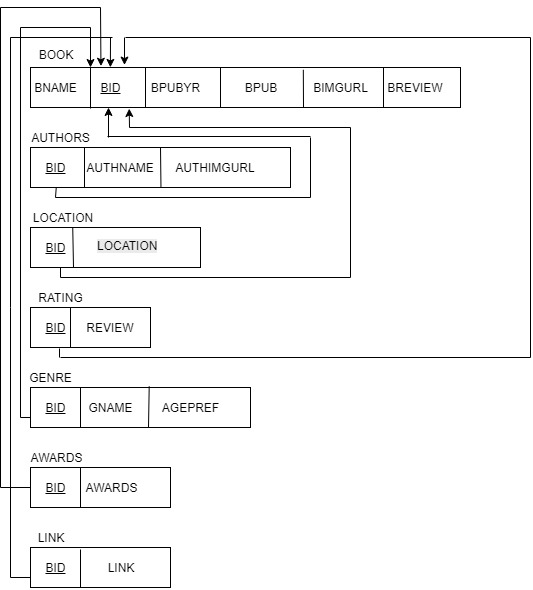
\includegraphics[scale=.5]{./tschema.jpg}
\\[0.2in]
\label{fig:Relational Schema}
\end{figure}

\thispagestyle{fancy}
\chapter{DESCRIPTION OF TOOLS AND TECHNOLOGIES}
\section{Microsoft visual Studio}
Microsoft Visual Studio is an integrated development environment(IDE) from Microsoft. It is used to develop console and graphical user interface applications along with Windows Form applications, websites, web applications, and web services in both native code together with managed code for all platforms supported by Microsoft Window, Windows Mobile, Windows CE, .NET Framework, .NET Compact Framework and Microsoft Silverlight. Microsoft Visual Studio simplifies the basic tasks of creating, debugging and deploying applications.
Microsoft Visual Studio comes with .NET Framework and supports applications targeting Windows. It supports IBM DB2 and Oracle databases, in addition to Microsoft SQL Server. It has integrated support for developing Microsoft Silverlight applications, including an interactive designer. Microsoft Visual Studio offers several tools to make parallel programming simpler: in addition to the Parallel Extensions for the .NET Framework and the Parallel Patterns Library for native code, Visual Studio includes fools for debugging parallel applications.
The Visual Studio code editor now highlights references; whenever a symbol is selected; all other usages of the symbol are highlighted. It also offers a Quick Search feature to incrementally search across all symbols in C++, Csharp and VB.NET projects. Quick Search supports substring matches and camel Case searches. The Call Hierarchy feature allows the developers to see all the methods that are called from a current method as well as the methods that call the current one. IntelliSense in Visual Studio supports a consume-first mode which developers can opt into. In this mode, IntelliSense will not auto-complete identifiers; this allows the developer to use undefined identifiers (like variable or method names) and define those later. Visual Studio can also help in this by automatically defining them, if it can infer their types from usage.
We have used Visual Studio Community 2015, v 14.0.23107.10 for developing the Inventory Management System Application.

\section{Microsoft SQL server Management Studio Express}
Microsoft SQL Server Management Studio Express (SSMSE) provides a graphical management tool for SQL Server Express Edition. SSMSE user interface is a subset of SQL Management Studio that is available with other editions of SQL Server. SSMSE call also manage instance of the SQL Server Database Engine created by any edition of SQL Server. Inventory Management System is developed using Microsoft SOL Server 2008.
\section{NET Framework 4.5}
The .NET Framework is a development platform for building apps for Windows, Windows Phone, Windows Server, and Microsoft Azure. It consists of the common language runtime (CLR) and the .NET Framework class library, which includes classes, interfaces, and value types that support an extensive range of technologies. The .NET Framework provides a managed execution environment, simplified development and deployment, and integration with a variety of programming languages, including Visual Basic and Visual Cshrap.
\section{.NET Framework Structure}
The .Net architecture is basically segregated in to three layers namely top, middle and bottom layer. The bottom layer is CLR, it is the heart of .NET Framework which provides the runtime environment in which programs are executed. The middle layer comprises the next generation of standard system services are brought under the control of the framework, making them universally available and standardizing their usage across languages.
\section{The .NET Language}
In the past, you chose the development language for an application based upon the functionality that you were trying to perform. Some languages were more powerful than others, but at the same time they might have required a higher level of understanding and were, in most cases, more difficult to program in.Now the .NET Framework provides you with a language-independent programming platform. You do not have to decide which language would provide a better solution. All languages are now on a level playing field. In .NET, no one language is superior to any of the other languages. They all have equal access to everything that .NET offers.
To be part of the .NET Framework, a language only has to follow certain rules. The biggest and most important rule for inclusion is that the language needs to be an object-oriented language. Microsoft provides four languages with the .NET Framework:
Visual Basic .NET
Csharp
C++.NET and
Jscript .NET.
Microsoft also provides Jsharp (pronounced J-sharp), but in order to use this new language that is basically Java for .NET, you need to download the language to install it on your server.
Data Provider:
The data provider is responsible for providing and maintaining the connection to the database. A database provider is a set of related components that works together to provide in an efficient and performance driven manner. Each Data provider consists of the following components classes:
 The command object which is used to execute a command.
 The Connection object which provides a connection to the database.
 The Data Reader object which provides a ready only, connects recordset.
\section{The Connection object}
The connection object created the connection to the database. Microsoft Visual Studio .NET provides two types of connection classes: the SQLconnection object, which is designed specifically to connect to Microsoft SQL Server.
\section{The command Object}
The command object is represented by corresponding classes: SQL Command. Command object are used to execute commands to a database across a data connection. The command objects provides three methods that are used to execute commands on the database.
19
 ExecuteNonQuery: Executes commands that have no return values such as INSERT, UPDATE AND DELETE
 ExecuteScalar: Returns a single value from a database query
 ExecuteReader: Returns a result set by way of a DataReader Objects.
\section{The Data Reader object}
The DataReadre object provides a read-only, connected stream recordset from a database. Unlike other components of the Data Provider, DataReader objects cannot be directly instantiated. Rather, the DateReader is returned as the result of the Command objectsExecute Reader method. The DataReader can provide rows of data directly to application logic when one does not need to keep the data cached in memory. Because only one row is in memory in time, the DateReader provides the lowest overhead in terms of system performance but requires the exclusive use of an open Connection object for the life time of the DataReader.
\section{Microsoft SQL Server}
Microsoft SQL Server is an application used to create computer databases for the Microsoft Windows family of server operating systems. Microsoft SQL Server provides an environment used to generate database that can be accessed from workstations, the Internet, or other media such as a personal digital assistant (PDA). Microsoft SQL Server is used to create desktop, enterprise, and web-based database applications. It is used at different levels and with various goals.
SQL Server makes simpler and easier to deploy, manage, and optimize enterprise data and analytical applications. An enterprise data management platform, it performs a single management console that enables data administrators anywhere in your organization to monitor, manage, and tune all of the databases and associated services across your enterprise. It provides an extensible management infrastructure that can be easily programmed by using SQL management objects, enabling users to customize and extend their management environment and independent software vendors to build additional tools and functionality to further extend the capabilities that come out of the box.
SQL Server simplifies management by providing integrated management console to monitor and manage the SQL Server relational database as well as integration services, analysis services, reporting services, notification services and SQL Server Mobile Edition across large number of distributed servers and databases. Databaseadministrator can perform several tasks at the same time, such as authorizing and executing a query, viewing server objects, managing an object, monitoring system activities, and viewing online help.
SQL Server expose more than 70 new measures of internal database performance and resource usages, ranging from memory, locking, and scheduling to transactions and network and disk I/O. these dynamic management views provide greater transparency and visibility into the database and a powerful infrastructure for proactive monitoring of database health and performance. The major characteristics are listed below:
Reliability: achieve a more secure deployment. SQL Server provides rich security features to protect data and network resources.
Confidentiality: Protect your data. SQL Server clustering supports Kerberos authentication on a virtual Server and Microsoft-style policies on standard logins so that a consistent policy is applied across all accounts in the domain.
Integrity: SQL Server supports encryption capabilities within database itself, fully integrated with a key management infrastructure. By default, client server communications are in encrypted.administrator can perform several tasks at the same time, such as authorizing and executing a query, viewing server objects, managing an object, monitoring system activities, and viewing online help.
SQL Server expose more than 70 new measures of internal database performance and resource usages, ranging from memory, locking, and scheduling to transactions and network and disk I/O. these dynamic management views provide greater transparency and visibility into the database and a powerful infrastructure for proactive monitoring of database health and performance. The major characteristics are listed below:
Reliability: achieve a more secure deployment. SQL Server provides rich security features to protect data and network resources.
Confidentiality: Protect your data. SQL Server clustering supports Kerberos authentication on a virtual Server and Microsoft-style policies on standard logins so that a consistent policy is applied across all accounts in the domain.
Integrity: SQL Server supports encryption capabilities within database itself, fully integrated with a key management infrastructure. By default, client server communications are in encrypted.

\chapter{SQL Database Connectivity}
\section{The SqlConnection Object}
The first thing you will need to do when interacting with a database is to create a connection. The connection tells the rest of the .NET code which database it is talking to. It manages all of the low-level logic associated with the specific database protocols. This makes it easy for you because the most work you will have to do in code instantiates the connection object, open the connection, and then close the connection when you are done. 
\section{Creating a SqlConnection Object}
\begin{lstlisting}
A SqlConnection is an object, just like any other C# object.  Most of the time, you just declare and instantiate the SqlConnection all at the same time, as shown below:
SqlConnection con = new SqlConnection(@"Data Source = (LocalDB)\MSSQLLocalDB; AttachDbFilename=|DataDirectory|\Database1.mdf;Integrated Security = True");
The SqlConnection object instantiated above uses a constructor with a single argument of type string This argument is called a connection string.
\end{lstlisting} 
\section{The SqlCommand Object}
A SqlCommand object allows you to specify what type of interaction you want to perform with a database. For example, you can do select, insert, modify, and delete commands on rows of data in a database table. The SqlCommand object can be used to support disconnected data management scenarios, but in this lesson, we will only use the SqlCommand object alone. A later lesson on the SqlDataAdapter will explain how to implement an application that uses disconnected data. This lesson will also show you how to retrieve a single value from a database, such as the number of records in a table. 
\section{Creating a SqlCommand Object}
\begin{lstlisting}
Similar to other Csharp objects, you instantiate a Sql Command object via the new instance declaration, as follows:
SqlCommand cmd = new SqlCommand("rating_sp", con);  
The line above is typical for instantiating a Sql Command object. It takes a string parameter that holds the command you want to execute and a reference to a Sql Connection object.
\end{lstlisting}



\chapter{Implementation}
\section{FORMS}
\subsection{Home Page}
\begin{lstlisting}
using System;
using System.Collections.Generic;
using System.ComponentModel;
using System.Data;
using System.Drawing;
using System.Linq;
using System.Text;
using System.Threading.Tasks;
using System.Windows.Forms;


namespace BookCataloguing
{
    public partial class Form1 : Form
    {
        Form2 f2 = new Form2();
        Form3 f3 = new Form3();
        Form4 f4 = new Form4();
        Form5 f5 = new Form5();
        Form6 f6 = new Form6();
        Form7 f7 = new Form7();
        Form8 f8 = new Form8();
        Form9 f9 = new Form9();

        public Form1()
        {
            InitializeComponent();
        }

        private void button1_Click(object sender, EventArgs e)
        {
            try
            {
                f2.ShowDialog();
            }
            catch(Exception exception)
            {
                new Form2().ShowDialog();
            }
           

        }

        

        private void button2_Click_1(object sender, EventArgs e)
        {
            try
            {
                f3.ShowDialog();
            }
            catch (Exception exceptio)
            {
                new Form3().ShowDialog();
            }
        }

        private void button3_Click_1(object sender, EventArgs e)
        {
            try
            {
                f4.ShowDialog();
            }
            catch (Exception exceptin)
            {
                new Form4().ShowDialog();
            }
        }

        private void button4_Click_1(object sender, EventArgs e)
        {
            try
            {
                f5.ShowDialog();
            }
            catch (Exception excepton)
            {
                new Form5().ShowDialog();
            }
        }


        private void button6_Click(object sender, EventArgs e)
        {
            try
            {
                f6.ShowDialog();
            }
            catch (Exception exception)
            {
                new Form6().ShowDialog();
            }
        }

        private void button8_Click(object sender, EventArgs e)
        {
            this.Close();
        }

        private void button5_Click(object sender, EventArgs e)
        {
           
        }

        private void button7_Click(object sender, EventArgs e)
        {
           
        }

        private void button10_Click(object sender, EventArgs e)
        {
            try
            {
                f8.ShowDialog();
            }
            catch (Exception xceptio)
            {
                new Form8().ShowDialog();
            }
        }

        private void button9_Click(object sender, EventArgs e)
        {
            try
            {
                f9.ShowDialog();
            }
            catch (Exception xceptio)
            {
                new Form9().ShowDialog();
            }
        }

        private void button5_Click_1(object sender, EventArgs e)
        {
            try
            {
                f7.ShowDialog();
            }
            catch (Exception exption)
            {
                new Form7().ShowDialog();
            }
        }

        private void button7_Click_1(object sender, EventArgs e)
        {
            this.Close();
        }
    }
}
\end{lstlisting}
\subsection{Book information}
\begin{lstlisting}
using System;
using System.Collections.Generic;
using System.ComponentModel;
using System.Data;
using System.Drawing;
using System.Linq;
using System.Text;
using System.Threading.Tasks;
using System.Windows.Forms;
using System.Data.SqlClient;
using System.Diagnostics;
namespace BookCataloguing
{
    public partial class Form2 : Form
    {

        SqlConnection con = new SqlConnection("Data Source=(LocalDB)\\MSSQLLocalDB;AttachDbFilename=|DataDirectory|\\Database1.mdf;Integrated Security=True");
        SqlCommand cmd;
        SqlDataReader Dr1;

        

        public void getauthrat()


        {
           
            
            con.Open();
             String b = label8.Text;

            string syntax = "SELECT a.authname, r.rating FROM authors a, rating r WHERE a.bid="+b+" and r.bid="+b;
            cmd = new SqlCommand(syntax, con);
            
            
                Dr1 = cmd.ExecuteReader();
                Dr1.Read();
                
            
           // catch(Exception e)
           // {
              //  MessageBox.Show("sql injection error");
            //}
            label3.Text = Dr1[0].ToString();
            label4.Text = Dr1[1].ToString();
            con.Close();
            // syntax = "";
        }

        public Form2()
        {
            InitializeComponent();
        }

       public void img()
        {
            string a = label7.Text;
            pictureBox1.ImageLocation = a;
            
        }
       
        
        private void button1_Click_1(object sender, EventArgs e)
        {
            this.Close();
        }

        private void Form2_Load(object sender, EventArgs e)
        {
            // TODO: This line of code loads data into the 'database1DataSet.location' table. You can move, or remove it, as needed.
            this.locationTableAdapter.Fill(this.database1DataSet.location);

            // TODO: This line of code loads data into the 'database1DataSet.book' table. You can move, or remove it, as needed.
            this.bookTableAdapter.Fill(this.database1DataSet.book);
           
           

        }

        private void button5_Click(object sender, EventArgs e)
        {
            con.Open();

            String b = label8.Text;
            string syntax = "SELECT buylink FROM link WHERE bid="+b;
            cmd = new SqlCommand(syntax, con);
            Dr1 = cmd.ExecuteReader();
            Dr1.Read();
            Process.Start(Dr1[0].ToString());
            
            con.Close();

        }

        

        private void listBox1_MouseMove(object sender, MouseEventArgs e)
        {
            img();
            getauthrat();
            Dr1.Equals("");
        }

        private void button3_Click(object sender, EventArgs e)
        {
            SqlDataReader Dr1;
            con.Open();

            String bidlink = label8.Text;
            string syntax = "SELECT location FROM location WHERE bid=" + bidlink;
            cmd = new SqlCommand(syntax, con);
            Dr1 = cmd.ExecuteReader();
            Dr1.Read();
            string loc = Dr1[0].ToString();
            loc.Trim();
            Process.Start(loc);
           
            con.Close();
            return;
        }

        private void label9_Click(object sender, EventArgs e)
        {

        }
    }
}
\end{lstlisting}
\subsection{Author page}
\begin{lstlisting}
using System;
using System.Collections.Generic;
using System.ComponentModel;
using System.Data;
using System.Drawing;
using System.Linq;
using System.Text;
using System.Threading.Tasks;
using System.Windows.Forms;
using System.Data.SqlClient;
namespace BookCataloguing
{
    public partial class Form3 : Form
    {
        SqlConnection con = new SqlConnection("Data Source=(LocalDB)\\MSSQLLocalDB;AttachDbFilename=|DataDirectory|\\Database1.mdf;Integrated Security=True");
        SqlCommand cmd;
        SqlDataReader Dr1;

        public Form3()
        {
            InitializeComponent();
        }
        public void bkld(object sender, EventArgs e)
        {
            try
            {
                cmd = new SqlCommand("auth1_SP", con);
                cmd.CommandType = CommandType.StoredProcedure;

                cmd.Parameters.AddWithValue("@authname", label1.Text);
                SqlDataAdapter DA = new SqlDataAdapter(cmd);
                DataSet DS = new DataSet();
                DA.Fill(DS);

                con.Open();
                try
                {
                    cmd.ExecuteNonQuery();


                }
                catch (Exception ex)
                {
                    MessageBox.Show("<<<INVALID SQL OPERATION>>> \n" + ex);

                }
                con.Close();

                dataGridView1.DataSource = DS.Tables[0];
                this.dataGridView1.Columns[0].AutoSizeMode = DataGridViewAutoSizeColumnMode.DisplayedCells;
                this.dataGridView1.Columns[1].AutoSizeMode = DataGridViewAutoSizeColumnMode.Fill;
               




            }
            catch (Exception ex)
            {
                MessageBox.Show(" " + ex);
            }
            

          //  String b = label3.Text;
           // string syntax = "SELECT authimgurl FROM authors WHERE bid=" + b; 
           // cmd = new SqlCommand(syntax, con);


           // Dr1 = cmd.ExecuteReader();
          //  Dr1.Read();


           
           // label2.Text = Dr1[0].ToString();
           
            
            pictureBox1.ImageLocation = label2.Text;

        }




        private void button2_Click_1(object sender, EventArgs e)
        {
            this.Close();
        }

        private void button1_Click(object sender, EventArgs e)
        {
            
        }

        private void Form3_Load(object sender, EventArgs e)
        {
            // TODO: This line of code loads data into the 'database1DataSet1.authors' table. You can move, or remove it, as needed.
            this.authorsTableAdapter1.Fill(this.database1DataSet1.authors);
            // TODO: This line of code loads data into the 'database1DataSet.authors' table. You can move, or remove it, as needed.
            this.authorsTableAdapter.Fill(this.database1DataSet.authors);

        }

        private void listBox1_MouseMove(object sender, MouseEventArgs e)
        {
            string a = label2.Text;
            pictureBox1.ImageLocation = a;
            try
            {
                cmd = new SqlCommand("auth1_SP", con);
                cmd.CommandType = CommandType.StoredProcedure;

                cmd.Parameters.AddWithValue("@authname", label1.Text);
                SqlDataAdapter DA = new SqlDataAdapter(cmd);
                DataSet DS = new DataSet();
                DA.Fill(DS);

                con.Open();
                try
                {
                    cmd.ExecuteNonQuery();


                }
                catch (Exception ex)
                {
                    MessageBox.Show("<<<INVALID SQL OPERATION>>> \n" + ex);

                }
                con.Close();

                dataGridView1.DataSource = DS.Tables[0];
                this.dataGridView1.Columns[0].AutoSizeMode = DataGridViewAutoSizeColumnMode.DisplayedCells;
                this.dataGridView1.Columns[1].AutoSizeMode = DataGridViewAutoSizeColumnMode.Fill;

               



            }
            catch (Exception ex)
            {
                MessageBox.Show(" " + ex);
            }

        }
    }
}
\end{lstlisting}
\subsection{Genre page}
\begin{lstlisting}
using System;
using System.Collections.Generic;
using System.ComponentModel;
using System.Data;
using System.Drawing;
using System.Linq;
using System.Text;
using System.Threading.Tasks;
using System.Windows.Forms;
using System.Data.SqlClient;

namespace BookCataloguing
{
    public partial class Form4 : Form
    {
        SqlConnection con = new SqlConnection("Data Source=(LocalDB)\\MSSQLLocalDB;AttachDbFilename=|DataDirectory|\\Database1.mdf;Integrated Security=True");
        SqlCommand cmd;
        public Form4()
        {
            InitializeComponent();
        }

        private void button2_Click_1(object sender, EventArgs e)
        {
            this.Close();
        }

        private void button1_Click(object sender, EventArgs e)

        {
            try
            {
                cmd = new SqlCommand("gen_sp", con);
                cmd.CommandType = CommandType.StoredProcedure;

                cmd.Parameters.AddWithValue("@gname", textBox1.Text);
                SqlDataAdapter DA = new SqlDataAdapter(cmd);
                DataSet DS = new DataSet();
                DA.Fill(DS);

                con.Open();
                try
                {
                    cmd.ExecuteNonQuery();


                }
                catch (Exception ex)
                {
                    MessageBox.Show("<<<INVALID SQL OPERATION>>> \n" + ex);

                }
                con.Close();

                dataGridView1.DataSource = DS.Tables[0];
                this.dataGridView1.Columns[0].AutoSizeMode = DataGridViewAutoSizeColumnMode.DisplayedCells;
                this.dataGridView1.Columns[1].AutoSizeMode = DataGridViewAutoSizeColumnMode.Fill;
                this.dataGridView1.Columns[2].AutoSizeMode = DataGridViewAutoSizeColumnMode.DisplayedCells;




            }
            catch (Exception ex)
            {
                MessageBox.Show(" " + ex);
            }

        }

        private void panel4_Paint(object sender, PaintEventArgs e)
        {

        }

        private void button7_Click(object sender, EventArgs e)
        {

        }

        private void button2_Click(object sender, EventArgs e)
        {
            this.Close();
        }
    }
}


\end{lstlisting}
\subsection{Award page}
\begin{lstlisting}
using System;
using System.Collections.Generic;
using System.ComponentModel;
using System.Data;
using System.Data.SqlClient;
using System.Drawing;
using System.Linq;
using System.Text;
using System.Threading.Tasks;
using System.Windows.Forms;

namespace BookCataloguing
{
    public partial class Form5 : Form
    {
        SqlConnection con = new SqlConnection("Data Source=(LocalDB)\\MSSQLLocalDB;AttachDbFilename=|DataDirectory|\\Database1.mdf;Integrated Security=True");
        SqlCommand cmd;
        public Form5()
        {
            InitializeComponent();
        }

        

        private void button2_Click_1(object sender, EventArgs e)
        {
            this.Close();
        }

        private void Form5_Load(object sender, EventArgs e)
        {
            // TODO: This line of code loads data into the 'database1DataSet.awards' table. You can move, or remove it, as needed.
            this.awardsTableAdapter.Fill(this.database1DataSet.awards);
            

        }

        private void button1_Click(object sender, EventArgs e)
        {
            try
            {
                cmd = new SqlCommand("awards_sp", con);
                cmd.CommandType = CommandType.StoredProcedure;

                cmd.Parameters.AddWithValue("@awards", comboBox1.Text);
                SqlDataAdapter DA = new SqlDataAdapter(cmd);
                DataSet DS = new DataSet();
                DA.Fill(DS);

                con.Open();
                try
                {
                    cmd.ExecuteNonQuery();


                }
                catch (Exception ex)
                {
                    MessageBox.Show("<<<INVALID SQL OPERATION>>> \n" + ex);

                }
                con.Close();

                dataGridView1.DataSource = DS.Tables[0];
                this.dataGridView1.Columns[0].AutoSizeMode = DataGridViewAutoSizeColumnMode.DisplayedCells;
                this.dataGridView1.Columns[1].AutoSizeMode = DataGridViewAutoSizeColumnMode.Fill;
                




            }
           catch (Exception ex)
           {
                MessageBox.Show(" " + "ok");
            }
        }

        private void button2_Click(object sender, EventArgs e)
        {
            this.Close();
        }

        private void comboBox1_SelectedIndexChanged(object sender, EventArgs e)
        {

        }

        private void fillByToolStripButton_Click(object sender, EventArgs e)
        {
            try
            {
                this.awardsTableAdapter.FillBy(this.database1DataSet.awards);
            }
            catch (System.Exception ex)
            {
                System.Windows.Forms.MessageBox.Show(ex.Message);
            }

        }

        private void button2_Click_2(object sender, EventArgs e)
        {
            this.Close();
        }
    }
}
\end{lstlisting}
\subsection{Rating page}
\begin{lstlisting}
using System;
using System.Collections.Generic;
using System.ComponentModel;
using System.Data;
using System.Drawing;
using System.Linq;
using System.Text;
using System.Threading.Tasks;
using System.Windows.Forms;
using System.Data.SqlClient;
namespace BookCataloguing
{
    public partial class Form6 : Form
    {
        SqlConnection con = new SqlConnection("Data Source=(LocalDB)\\MSSQLLocalDB;AttachDbFilename=|DataDirectory|\\Database1.mdf;Integrated Security=True");
        SqlCommand cmd;
        public Form6()
        {
            InitializeComponent();
        }

        private void button2_Click(object sender, EventArgs e)
        {
            this.Close();

        }

        private void panel4_Paint(object sender, PaintEventArgs e)
        {

        }

        private void button5_Click(object sender, EventArgs e)
        {
            try
            {
                SqlCommand cmd = new SqlCommand("rating_sp", con);
                cmd.CommandType = CommandType.StoredProcedure;

                cmd.Parameters.AddWithValue("@rating", textBox1.Text);
                SqlDataAdapter DA = new SqlDataAdapter(cmd);
                DataSet DS = new DataSet();
                DA.Fill(DS);

                con.Open();
                try
                {
                    cmd.ExecuteNonQuery();


                }
                catch (Exception ex)
                {
                    MessageBox.Show("<<<INVALID SQL OPERATION>>> \n" + ex);

                }
                con.Close();

                dataGridView1.DataSource = DS.Tables[0];
                this.dataGridView1.Columns[0].AutoSizeMode = DataGridViewAutoSizeColumnMode.DisplayedCells;
                this.dataGridView1.Columns[1].AutoSizeMode = DataGridViewAutoSizeColumnMode.Fill;
                this.dataGridView1.Columns[2].AutoSizeMode = DataGridViewAutoSizeColumnMode.DisplayedCells;




            }
            catch (Exception ex)
            {
                MessageBox.Show(" " + ex);
            }

        }

        private void button2_Click_1(object sender, EventArgs e)
        {
            this.Close();
        }
    }
}
\end{lstlisting}
\subsection{Log page}
\begin{lstlisting}
using System;
using System.Collections.Generic;
using System.ComponentModel;
using System.Data;
using System.Drawing;
using System.Linq;
using System.Text;
using System.Threading.Tasks;
using System.Windows.Forms;

namespace BookCataloguing
{
    public partial class Form7 : Form
    {
        public Form7()
        {
            InitializeComponent();
        }

        private void Form7_Load(object sender, EventArgs e)
        {
            // TODO: This line of code loads data into the 'database1DataSet1.logdetails' table. You can move, or remove it, as needed.
            this.logdetailsTableAdapter.Fill(this.database1DataSet1.logdetails);

        }

        private void button2_Click(object sender, EventArgs e)
        {
            this.Close();
        }

      
    }
}
\end{lstlisting}
\subsection{Insert page}
\begin{lstlisting}
using System;
using System.Collections.Generic;
using System.ComponentModel;
using System.Data;
using System.Data.SqlClient;
using System.Drawing;
using System.Linq;
using System.Text;
using System.Threading.Tasks;
using System.Windows.Forms;

namespace BookCataloguing
{
    public partial class Form8 : Form
    {
        
        public Form8()
        {
            InitializeComponent();
        }
        
        private void label4_Click(object sender, EventArgs e)
        {

        }

        private void button1_Click(object sender, EventArgs e)
        {
            SqlConnection con = new SqlConnection("Data Source=(LocalDB)\\MSSQLLocalDB;AttachDbFilename=|DataDirectory|\\Database1.mdf;Integrated Security=True");
            SqlCommand cmd = new SqlCommand("insert_SP", con);
            cmd.CommandType = CommandType.StoredProcedure;
            cmd.Parameters.AddWithValue("@bid", textBox14.Text);
            cmd.Parameters.AddWithValue("@bname", textBox1.Text);
            cmd.Parameters.AddWithValue("@bimgurl", textBox4.Text);
            cmd.Parameters.AddWithValue("@bpub", textBox9.Text);
            cmd.Parameters.AddWithValue("@bpubyr", textBox10.Text);
            cmd.Parameters.AddWithValue("@breview", textBox8.Text);
            cmd.Parameters.AddWithValue("@rating", textBox2.Text);

            cmd.Parameters.AddWithValue("@authname", textBox6.Text);
            cmd.Parameters.AddWithValue("@awards", textBox5.Text);
            cmd.Parameters.AddWithValue("@gname", textBox3.Text);
            cmd.Parameters.AddWithValue("@agepref", textBox13.Text);
            cmd.Parameters.AddWithValue("@buylink", textBox12.Text);
            cmd.Parameters.AddWithValue("@location", textBox11.Text);
            cmd.Parameters.AddWithValue("@authimgurl", textBox7.Text);
            //  cmd.Parameters.AddWithValue("@", maskedTextBox13.Text);
            //  cmd.Parameters.AddWithValue("@rating", maskedTextBox13.Text);
            float rat=float.Parse(textBox2.Text);
            if (rat>5)
            {
                MessageBox.Show("ENTER RATING LESS THAN 5");
            }

            con.Open();
            try
            {
                if (rat > 5)
                {
                   // Form8 f8 = new Form8();
                    MessageBox.Show("ENTER RATING LESS THAN 5");
                    
                    new Form8().ShowDialog();
                    this.Close();
                    return;
                }
                cmd.ExecuteNonQuery();
                this.Close();
            }
            catch (Exception ex)
            {
                MessageBox.Show("    <<<<<INVALID SQL OPERATION>>>\n" + ex);
            }
            con.Close();
        }

        private void textBox1_TextChanged(object sender, EventArgs e)
        {

        }

        private void label11_Click(object sender, EventArgs e)
        {

        }

        private void label10_Click(object sender, EventArgs e)
        {

        }

        private void button2_Click(object sender, EventArgs e)
        {
            this.Close();
        }
    }
}
\end{lstlisting}
\subsection{Delete page}
\begin{lstlisting}
using System;
using System.Collections.Generic;
using System.ComponentModel;
using System.Data;
using System.Drawing;
using System.Linq;
using System.Text;
using System.Threading.Tasks;
using System.Windows.Forms;
using System.Data.SqlClient;

namespace BookCataloguing
{
    public partial class Form9 : Form
    {

        SqlConnection con = new SqlConnection("Data Source=(LocalDB)\\MSSQLLocalDB;AttachDbFilename=|DataDirectory|\\Database1.mdf;Integrated Security=True");
       
        SqlDataReader Dr1;

        public Form9()
        {
            InitializeComponent();
        }

        private void button1_Click(object sender, EventArgs e)
        {

        }

        private void Form9_Load(object sender, EventArgs e)
        {
            // TODO: This line of code loads data into the 'database1DataSet.book' table. You can move, or remove it, as needed.
            this.bookTableAdapter1.Fill(this.database1DataSet.book);
            // TODO: This line of code loads data into the 'database1DataSet1.book' table. You can move, or remove it, as needed.
            this.bookTableAdapter.Fill(this.database1DataSet1.book);
           
        }

        private void textBox1_TextChanged(object sender, EventArgs e)
        {

        }

        private void button3_Click(object sender, EventArgs e)
        {
            
            try
            {
               
               SqlCommand cmd = new SqlCommand("delete_sp", con);
                cmd.CommandType = CommandType.StoredProcedure;

                cmd.Parameters.AddWithValue("@bid", label3.Text);

                con.Open();
               
                try
                {
                    cmd.ExecuteNonQuery();
                }
                catch (Exception ex)
                {
                    MessageBox.Show("  <<<<<<<INVALID SQL OPERATION\n" + ex);
                }
                con.Close();
\end{lstlisting}

\section{STORED PROCEDURES}
\subsection{Book information related to a particular author}
\begin{lstlisting}
CREATE PROCEDURE [dbo].auth1_SP
	@authname nchar(50)
	
AS
	SELECT b.bname,a.authname from
	book b,authors a
	where a.authname=@authname and
	b.bid=a.bid
RETURN 0

\end{lstlisting}
\subsection{Book information related to a particular award}
\begin{lstlisting}
CREATE PROCEDURE [dbo].awards_sp
	@awards nchar(25)
AS
	SELECT b.bid,b.bname from 
	book b, awards a  where
	b.bid=a.bid and a.awards=@awards
RETURN 0
\end{lstlisting}
\subsection{Book information related to a particular genre}
\begin{lstlisting}
CREATE PROCEDURE [dbo].gen_sp
	@gname nchar(20)
AS
	SELECT b.bname,a.authname,g.gname
	from book b,authors a, genre g
	where b.bid=a.bid and b.bid=g.bid
	and g.gname=@gname
RETURN 0
\end{lstlisting}
\subsection{Book information based on rating}
\begin{lstlisting}
CREATE PROCEDURE [dbo].rating_sp
	@rating float
	
AS
	SELECT b.bname, r.rating, g.agepref FROM 
	book b, rating r, genre g WHERE b.bid=r.bid and b.bid=g.bid
	and r.rating>=@rating
RETURN 0
\end{lstlisting}
\subsection{Insert new book}
\begin{lstlisting}
CREATE PROCEDURE [dbo].insert_SP
	@bid int = 0,
	@authname nchar(50),
	@authimgurl varchar(200),
	@awards nchar(25),
	@bimgurl varchar(200),
	@bpub nchar(50),
	@bpubyr nchar(4),
	@breview varchar(MAX),
	@gname nchar(20),
	@agepref nchar(10),
	@buylink varchar(200),
	@location varchar(200),
	@rating float,


	@bname nchar(50)
	
AS
	insert into book(bid,bname,bimgurl,bpub,bpubyr,breview)values(@bid,@bname,@bimgurl,@bpub,@bpubyr,@breview)
	insert into rating(bid,rating)values(@bid,@rating)
	insert into authors(bid,authname,authimgurl)values(@bid,@authname,@authimgurl)
	insert into awards(bid,awards)values(@bid,@awards)
	insert into link(bid,buylink)values(@bid,@buylink)
	insert into location (bid,location)values(@bid,@location)
	insert into genre(bid,gname,agepref)values(@bid,@gname,@agepref)

RETURN 0
\end{lstlisting}
\subsection{Delete book}
\begin{lstlisting}
CREATE PROCEDURE [dbo].delete_sp
	@bid int 
	
AS
	DELETE FROM authors WHERE bid = @bid
	DELETE FROM awards WHERE bid = @bid
	DELETE FROM link WHERE bid = @bid
	DELETE FROM rating WHERE bid = @bid
	DELETE FROM genre WHERE bid = @bid
	DELETE FROM location WHERE bid = @bid
	DELETE FROM book WHERE bid = @bid
 RETURN 0
\end{lstlisting}
\section{TRIGGER}
\subsection{Log information of a book}
\begin{lstlisting}
CREATE TRIGGER tr_book_forinsert
	ON book
	FOR INSERT
	AS
	BEGIN
		SET NOCOUNT ON
		declare @booknm nchar(50)
		

		select @booknm = bname from inserted
		

		insert into logdetails values('Book with id'+cast(@booknm as nchar(50))+'inserted on'+ cast(GETDATE() as varchar(25)));
	END
\end{lstlisting}






\chapter{Snapshots}
\section{Home Page}
\begin{figure}[H]
\centering
\caption{HOME PAGE}
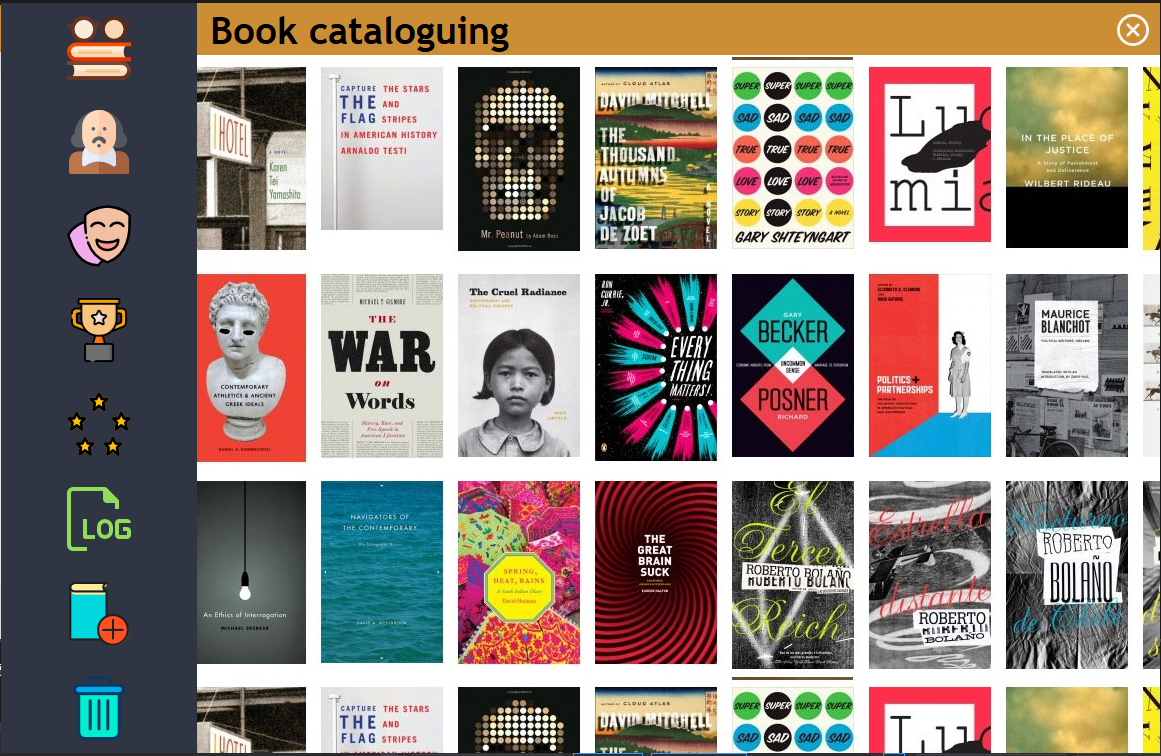
\includegraphics[scale=.5]{./sshome.png}
\\[0.2in]
\label{fig:HOME PAGE}
\end{figure}
\thispagestyle{fancy}
\section{Book information}
\begin{figure}[H]
\centering
\caption{BOOK INFORMATION}
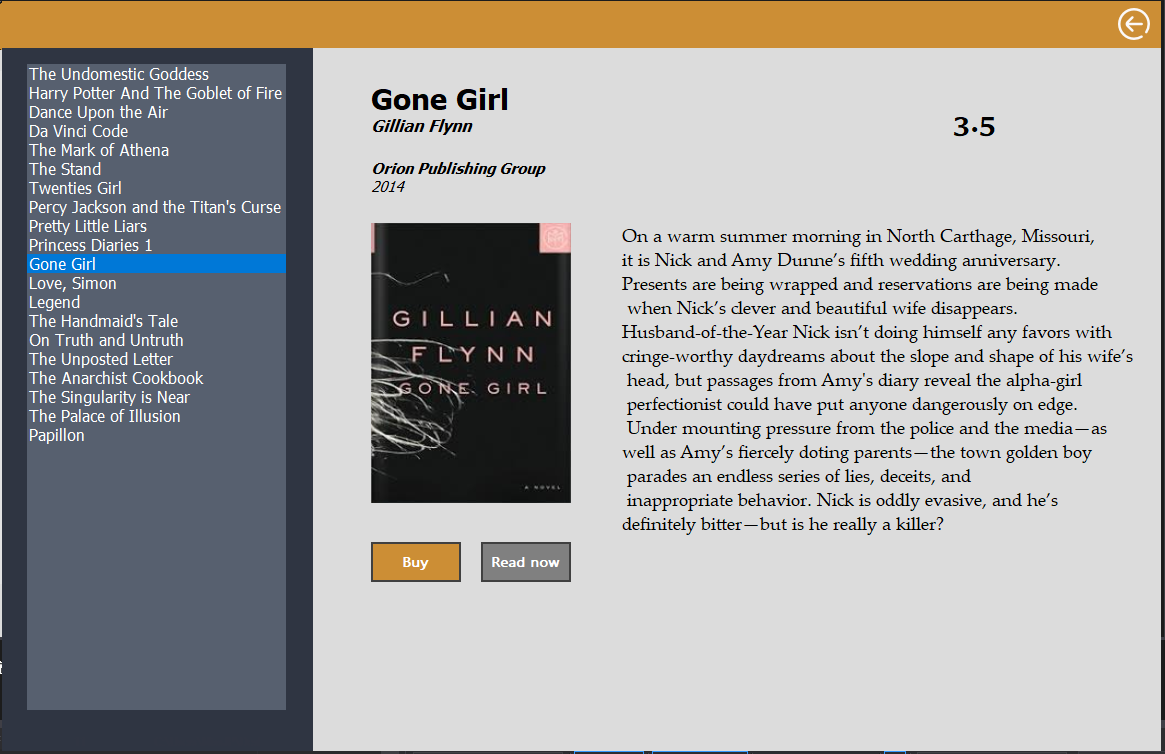
\includegraphics[scale=.5]{./ssbook.png}
\\[0.2in]
\label{fig:BOOK INFO}
\end{figure}
\thispagestyle{fancy}
\section{Author Page}
\begin{figure}[H]
\centering
\caption{AUTHOR PAGE}
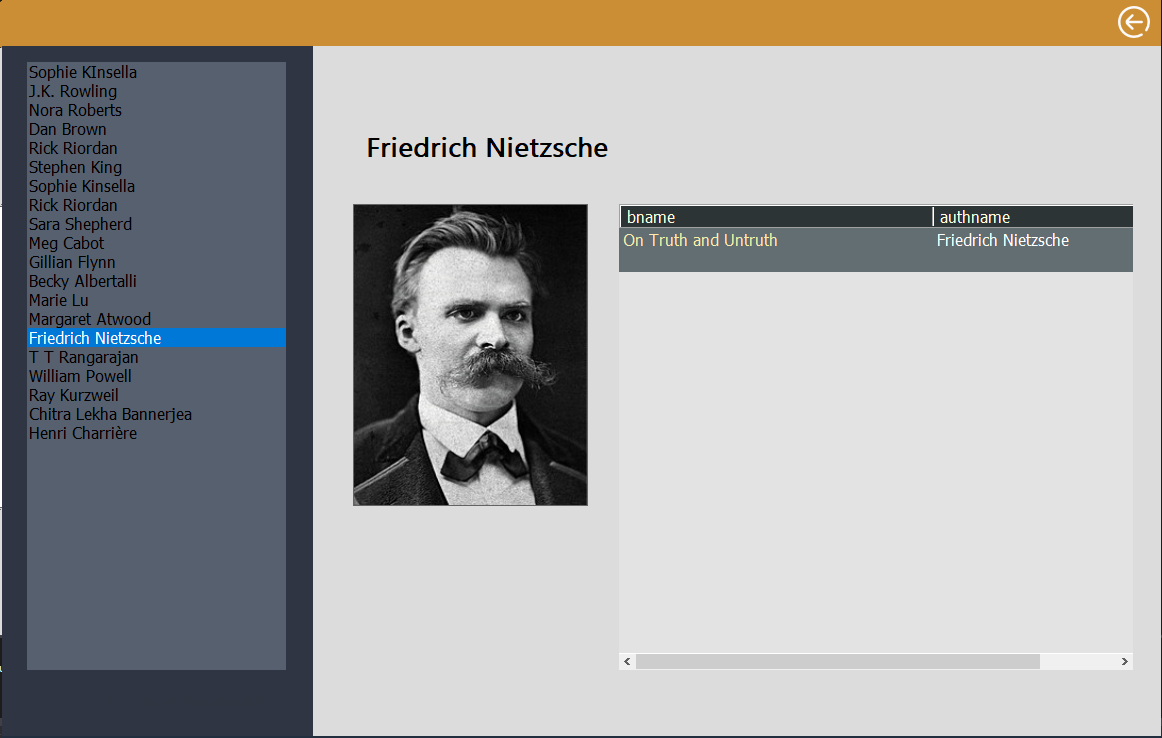
\includegraphics[scale=.5]{./ssauthors.png}
\\[0.2in]
\label{fig:auth}
\end{figure}
\thispagestyle{fancy}
\section{Awards Page}
\begin{figure}[H]
\centering
\caption{AWARDS PAGE 1}

\includegraphics[scale=.5]{./ssawards1.png}
\\[0.2in]
\label{fig:award}
\end{figure}
\thispagestyle{fancy}
\subsection{Select an award}
\begin{figure}[H]
\centering
\caption{AWARDS PAGE 2}
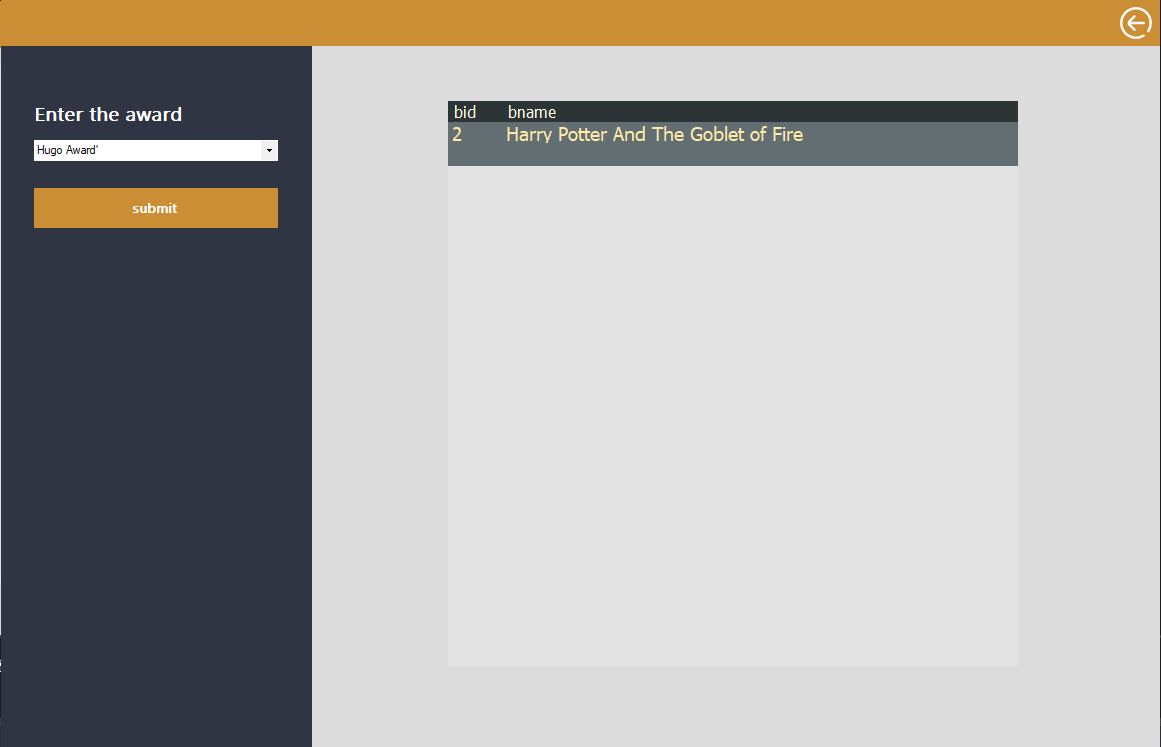
\includegraphics[scale=.5]{./ssawards2.png}
\\[0.2in]
\label{fig:award1}
\end{figure}
\thispagestyle{fancy}
\section{Genre Page}
\begin{figure}[H]
\centering
\caption{GENRE PAGE}
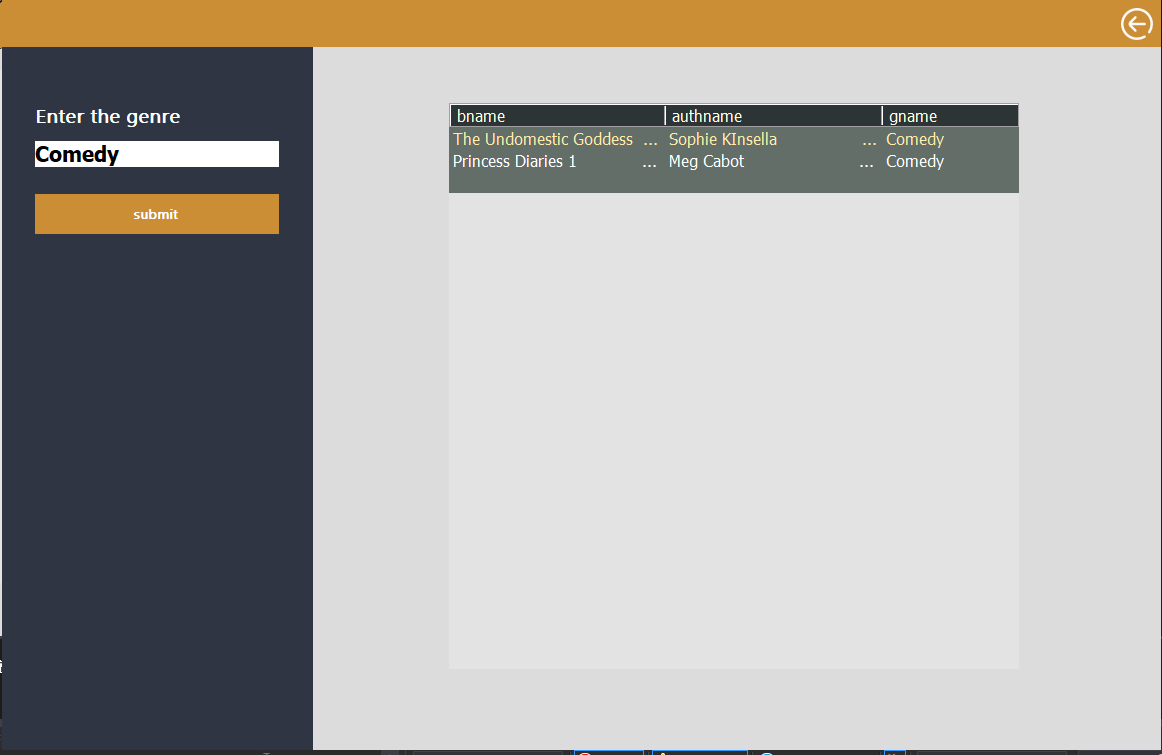
\includegraphics[scale=.5]{./ssgenre.png}
\\[0.2in]
\label{fig:genre}
\end{figure}
\thispagestyle{fancy}
\section{Rating Page}
\begin{figure}[H]
\centering
\caption{RATING PAGE}
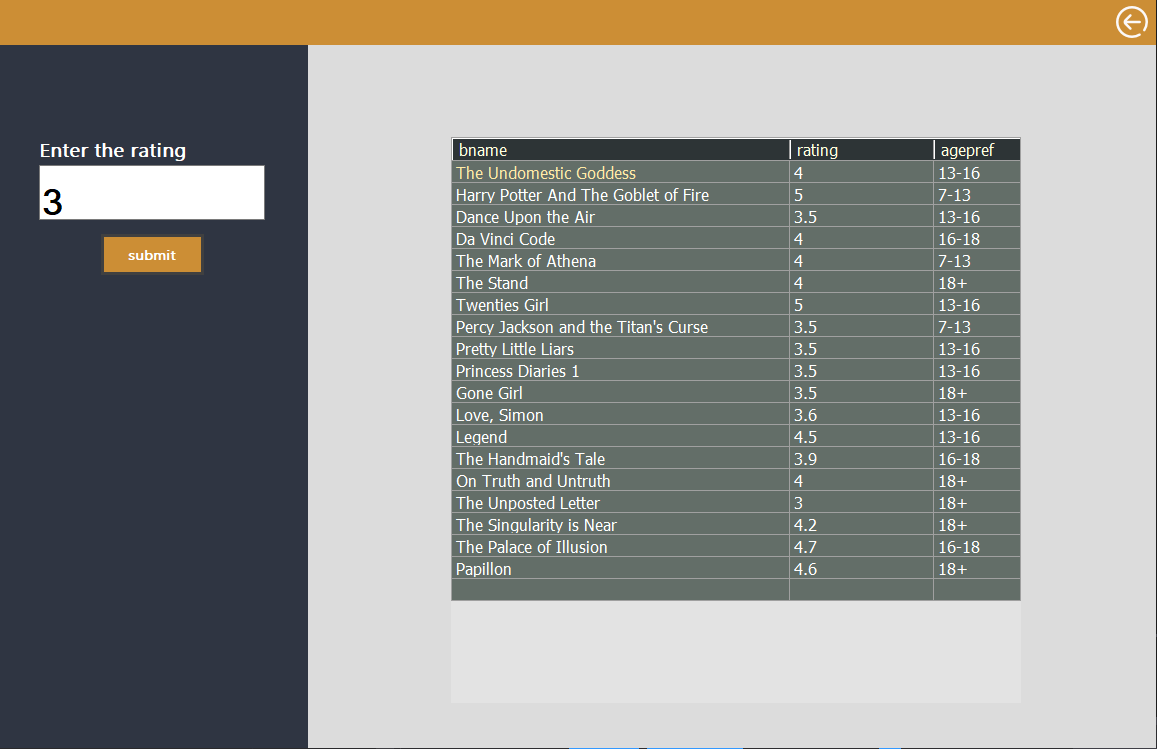
\includegraphics[scale=.5]{./ssrating.png}
\\[0.2in]
\label{fig:insert}
\end{figure}
\thispagestyle{fancy}
\section{Read-now Page}
\begin{figure}[H]
\centering
\caption{READ NOW PAGE}
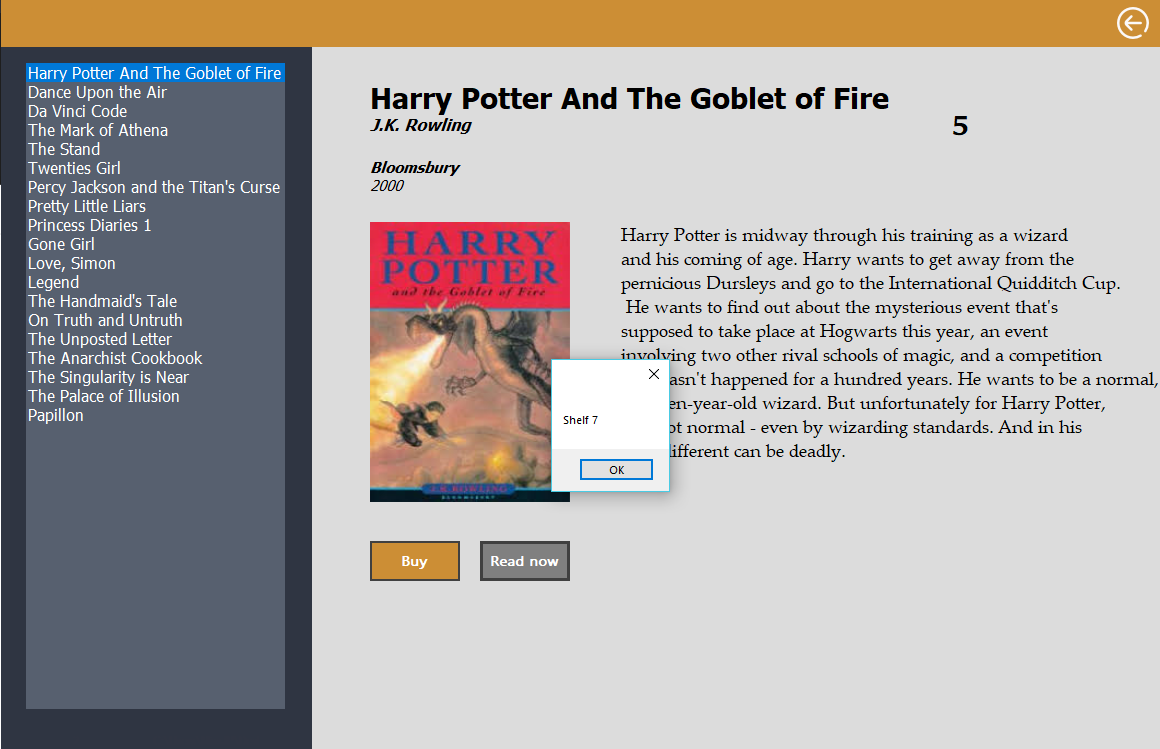
\includegraphics[scale=.5]{./ssreadnow.png}
\\[0.2in]
\label{fig:insert}
\end{figure}
\thispagestyle{fancy}
\section{Insert Page}
\begin{figure}[H]
\centering
\caption{INSERT PAGE 1}
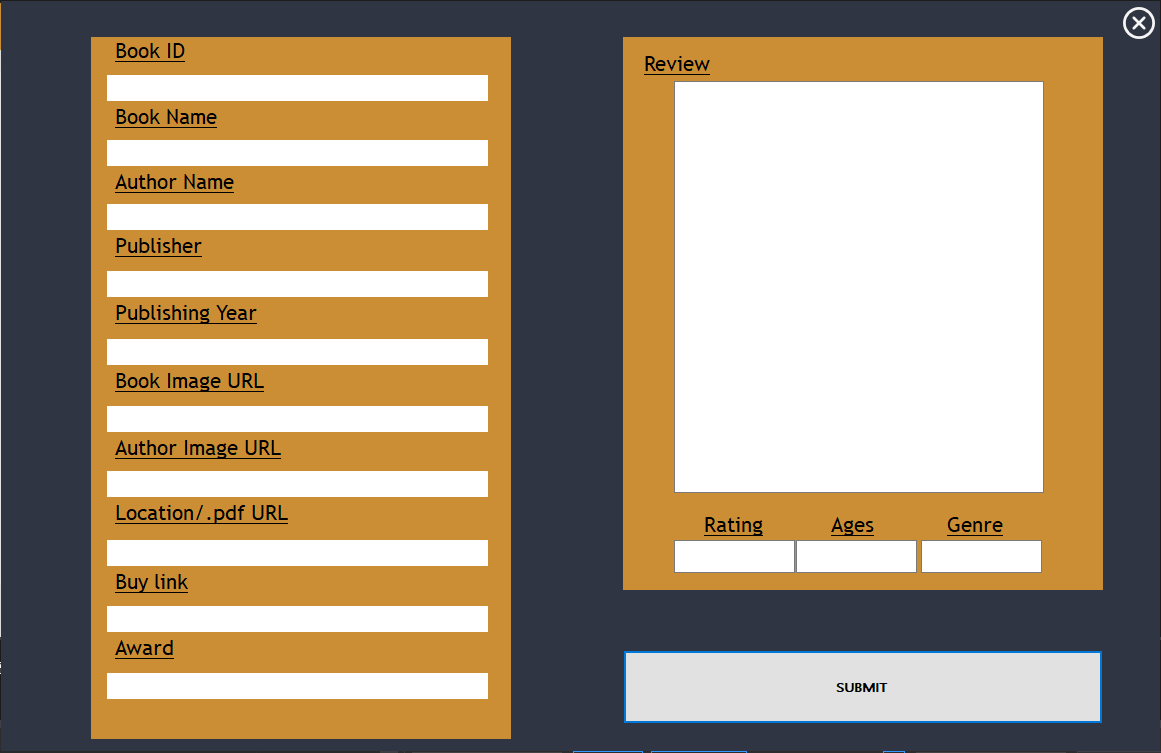
\includegraphics[scale=.5]{./ssinsert1.png}
\\[0.2in]
\label{fig:insert}
\end{figure}
\thispagestyle{fancy}
\subsection{Enter Information}
\begin{figure}[H]
\centering
\caption{INSERT PAGE 2}
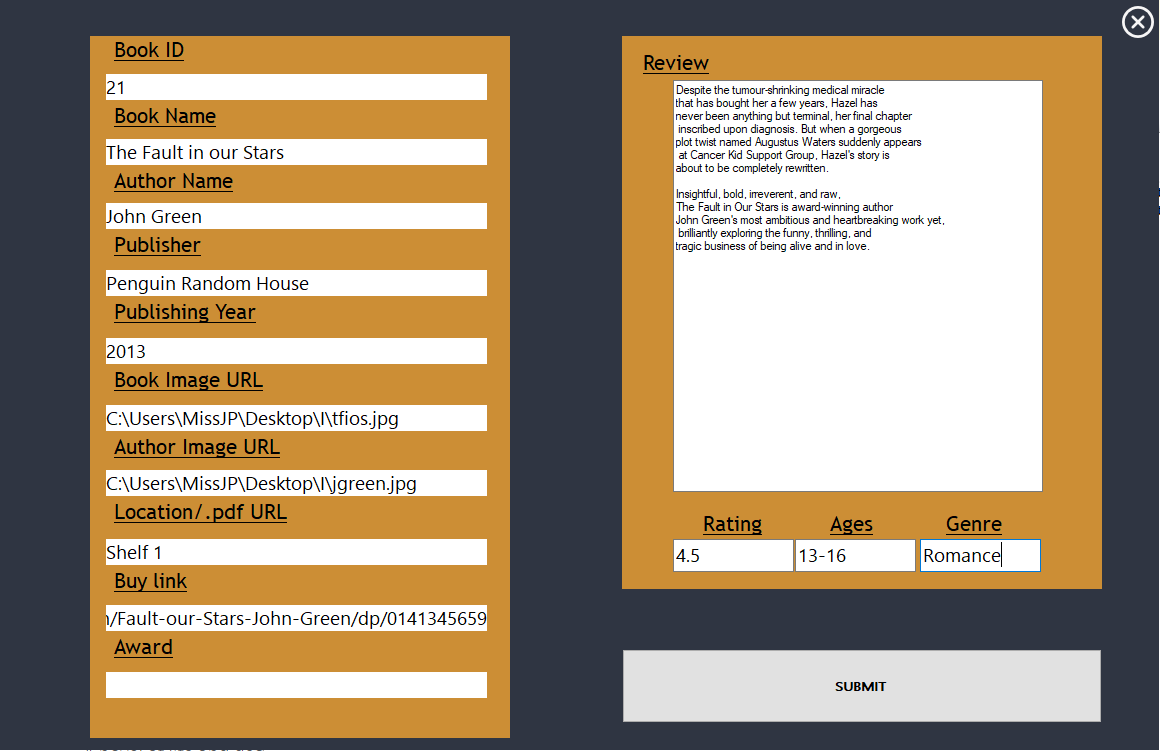
\includegraphics[scale=.5]{./ssinsert2.png}
\\[0.2in]
\label{fig:enter info}
\end{figure}
\thispagestyle{fancy}
\subsection{Book entered}
\begin{figure}[H]
\centering
\caption{INSERT PAGE 3}
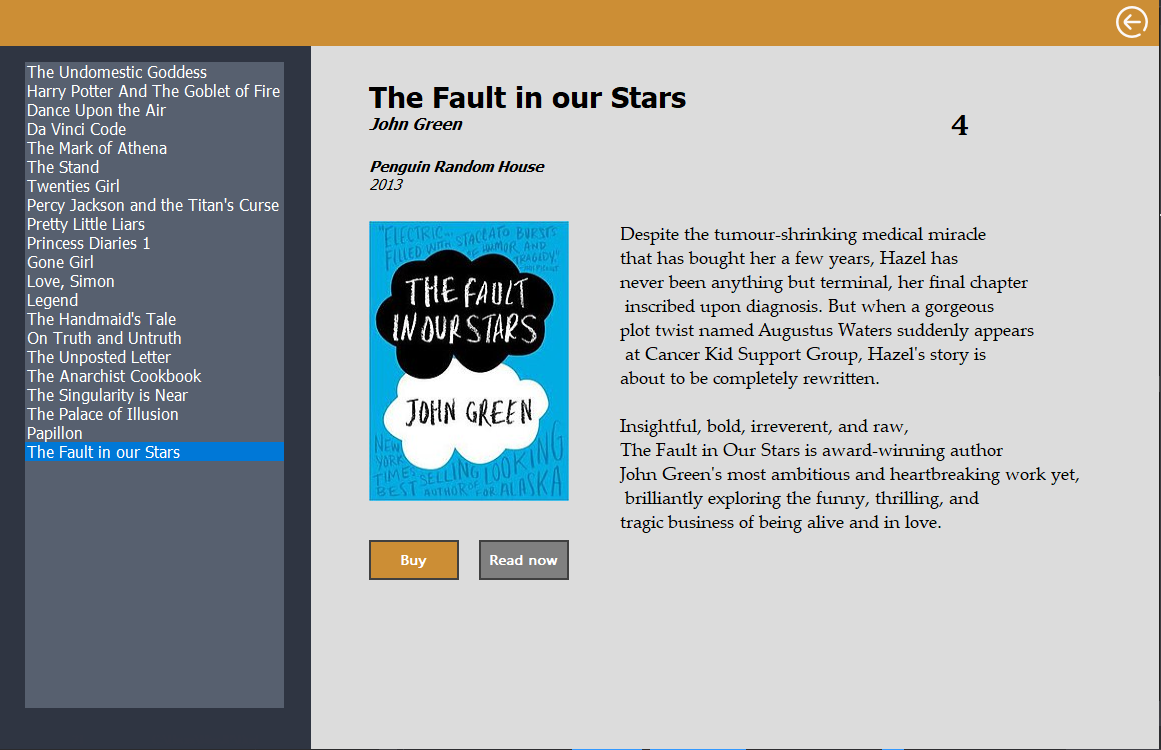
\includegraphics[scale=.5]{./ssinsert3.png}
\\[0.2in]
\label{fig:book ent}
\end{figure}
\thispagestyle{fancy}
\section{Delete Page}
\begin{figure}[H]
\centering
\caption{DELETE PAGE 1}
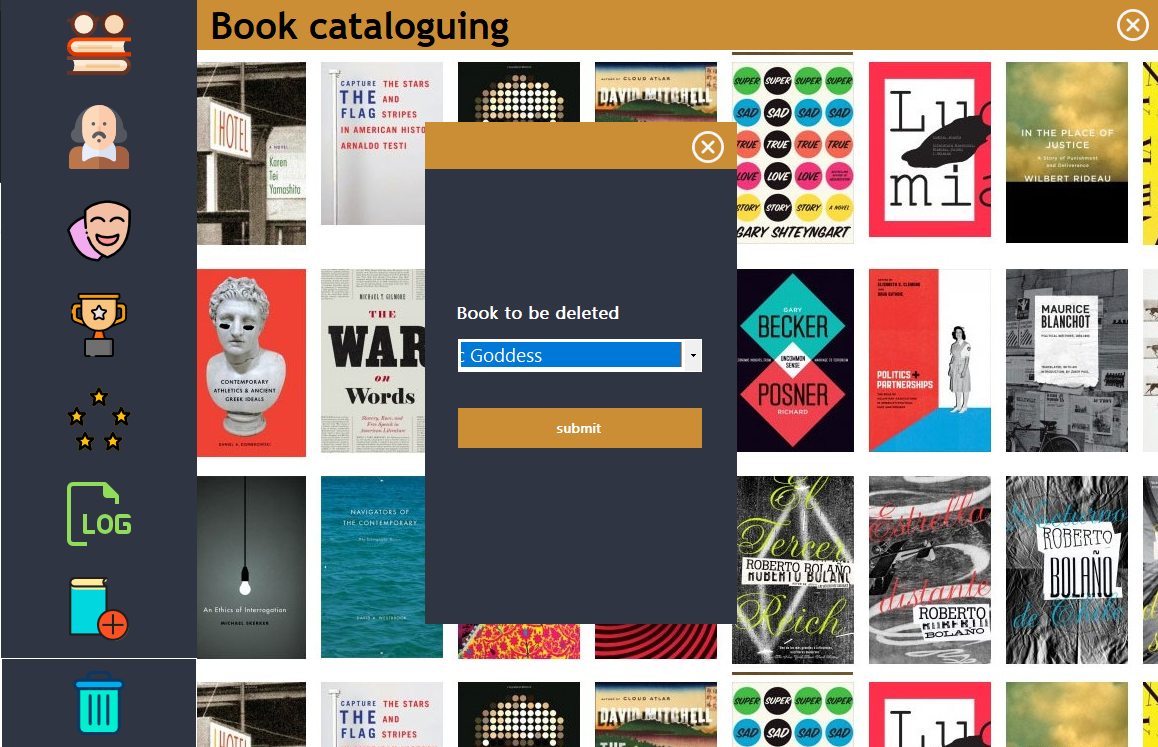
\includegraphics[scale=.5]{./ssdelete.png}
\\[0.2in]
\label{fig:del}
\end{figure}
\thispagestyle{fancy}\
\subsection{Book deleted}
\begin{figure}[H]
\centering
\caption{DELETE PAGE 2}
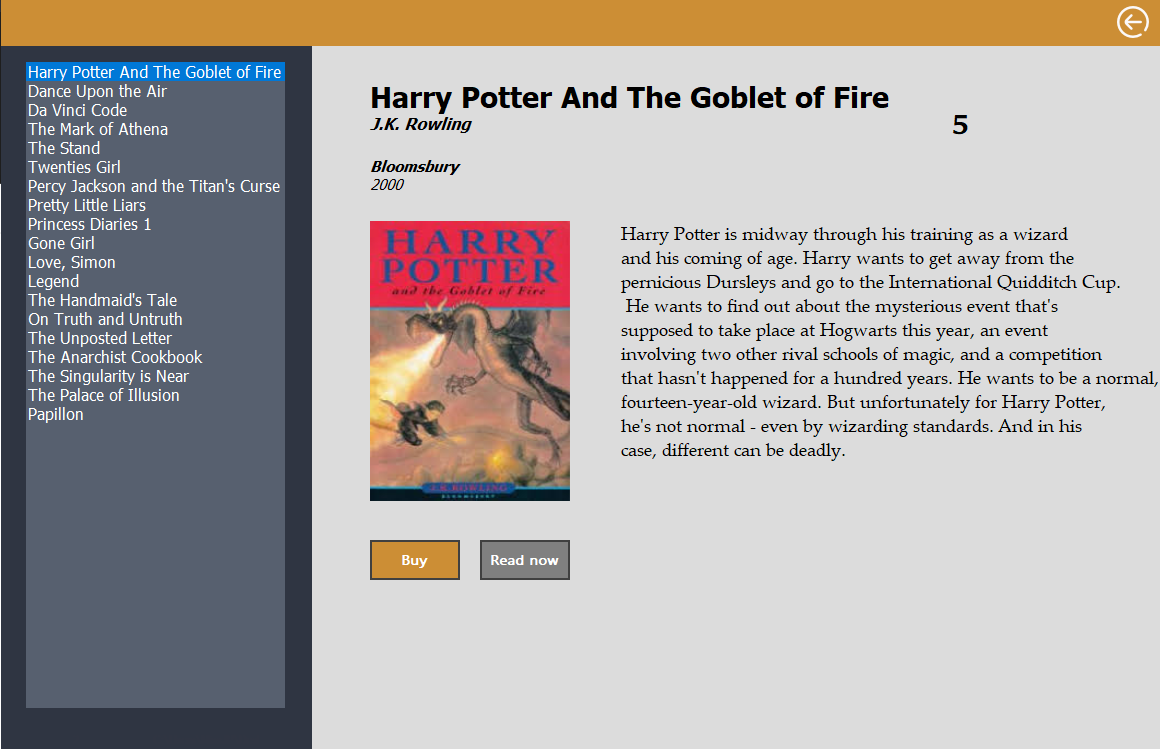
\includegraphics[scale=.5]{./ssdelete2.png}
\\[0.2in]
\label{fig:del2}
\end{figure}
\thispagestyle{fancy}
\section{Trigger Page}
\begin{figure}[H]
\centering
\caption{TRIGGER PAGE}
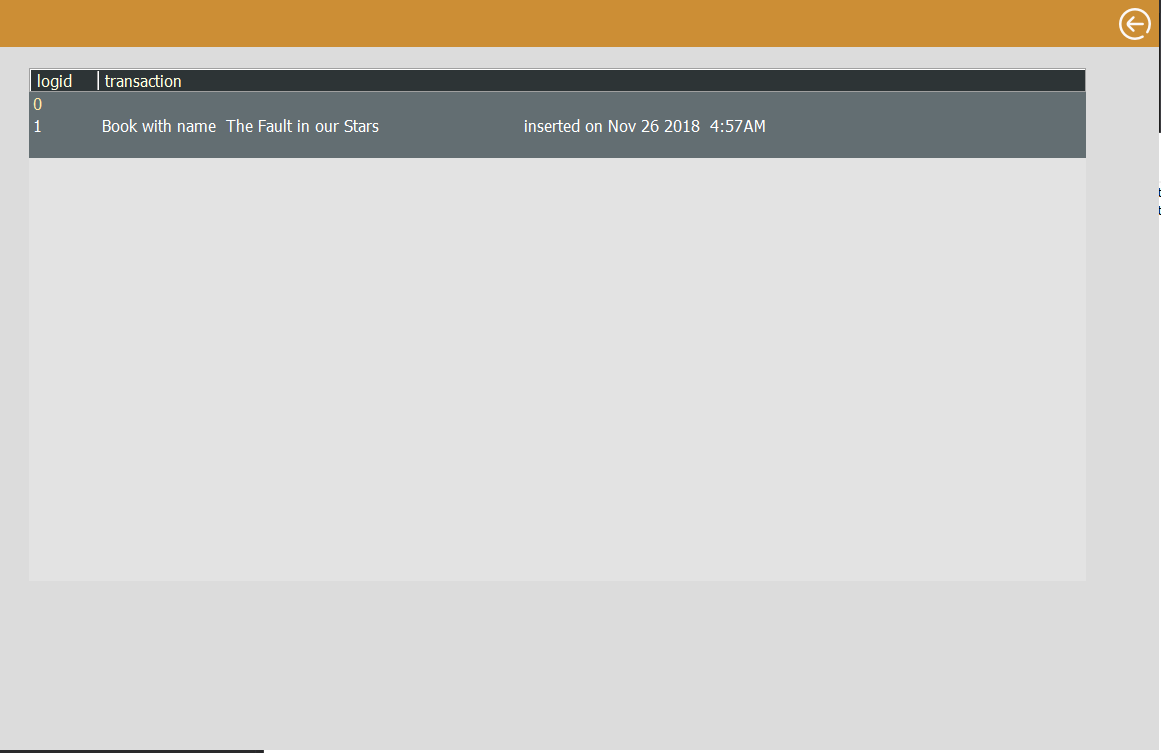
\includegraphics[scale=.5]{./ssinserttrigger.png}
\\[0.2in]
\label{fig:ER diagram}
\end{figure}
\thispagestyle{fancy}



\chapter{Conclusion and Future Enhancements}
This project is developed to minimize the chaos ensued and time consumed in managing a lot of books manually by an end user. This is done by embedding all the necessary data in a concise database and creating an apt interface. A future version of this project would incorporate multiple end users thus making this a social media. Suppose you have a spare hour or so in an airport and you want to do some light reading, this time is best spent reading and not choosing and searching for the book; here comes the book cataloguing system, this can be used to select an ebook after reading through the reviews. \\[0.2in]
The Book Cataloguing System is a rather personal project. I am an avid reader and wanted a tool to minimize my selection time and also a tool to store all the details of my personal book copies. I am thankful for being
provided this great opportunity to work on it.I am already implementing this to manage my books. As already mentioned, this project has gone through extensive research work. On the basis of the research work, we have successfully
designed and implemented The Book Cataloguing System. The world is becoming digital. Almost everything in the real world has it's counterpart in the virtual world. The Book Cataloguing system brings your personal book collection into the digital context.  \\[0.2in]

The most valuable future looks are following below:
\begin{itemize}

\item Having a globally accessible database of books so you can access it from anywhere.
\item A child safety feature that doesn't allow people under certain ages to access certain books
\item A social media pivot that makes this a place where people can review and rate books and add them to their shelves. A global marketplace for books.

\end{itemize}

\cleardoublepage
%\pagebreak
\phantomsection

\begin{thebibliography}{99}


\bibitem{} Learning Visual studio: \url{https://visualstudio.microsoft.com/}

\bibitem{} Additional help from\url{https://www.codeproject.com/}

\bibitem{} Doubts cleared from \url{https://stackoverflow.com/}
\end{thebibliography}



\end{document}


